\begin{abox}
	Electronics-Problems
	\end{abox}
\begin{enumerate}
	\item Calculate values of $V_{1}$ and $V_{2}$ across $4 \Omega$ and $5 \Omega$ resistor by KVL.
	\begin{figure}[H]
		\centering
		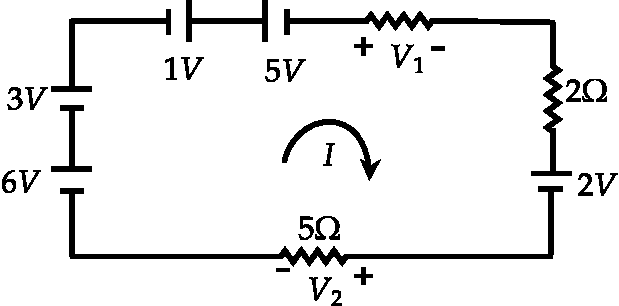
\includegraphics[height=3cm,width=6cm]{Ep-2}
	\end{figure}
	\begin{answer}
		\begin{align*}
		\text { Applying KVL }\\
		6+3+1-5-4 I-2 I-.2-5 I&=0\\
		3=111, \mathrm{I}&=\frac{3}{11} \mathrm{Amp}\\
		\mathrm{V}_{\mathrm{1}}=4 \mathrm{I}=4 \times \frac{3}{11} \mathrm{~V}&=\frac{12}{11} \text { volt }\\
		\mathrm{V}_{2}=-5 \mathrm{I}=-5 \times \frac{3}{11}&=-\frac{15}{11} \text { volt }
		\end{align*}
	\end{answer}
	\item Calculate $\mathrm{V}_{\mathrm{AB}}$ in the given circuit
	\begin{figure}[H]
		\centering
		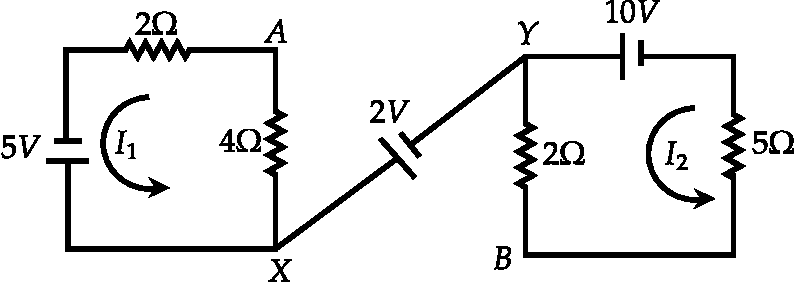
\includegraphics[height=2.8cm,width=7.5cm]{Ep-3}
	\end{figure}
	\begin{answer}
		\begin{align*}
		\mathrm{KVL} &\text { at loop 1: (Left loop) }\\
		-4 I_{1}-2 I_{1}+5&=0, \quad I_{1}=5 / 6 A m p\\
		\text { KVL at loop 2: }&\text{(Right loop) }\\
		10-2 I_{2}-5 I_{2}&=0\\
		\mathrm{I}_{2}=\frac{10}{7} \mathrm{Amp}, \mathrm{V}_{\mathrm{AB}}&=\mathrm{V}_{\mathrm{AX}}+\mathrm{V}_{\mathrm{XY}}+\mathrm{V}_{\mathrm{YB}}\\
		=-\frac{5}{6} \times 4+2+2 \times \frac{10}{7}&=-\frac{20}{6}+2+\frac{20}{7}=\frac{32}{21} V_{A B}=1.53 \text { Volt }
		\end{align*}
	\end{answer}
	\item The value of $I_{1}$ in the circuit is
	\begin{figure}[H]
		\centering
		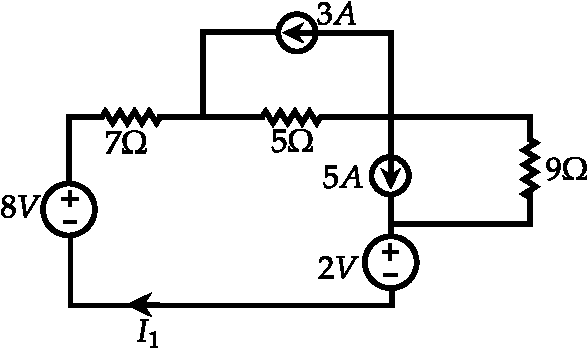
\includegraphics[height=3cm,width=5cm]{Ep-4}
	\end{figure}
	\begin{answer}$\left. \right. $
		The circuit can be redrawn in the form of voltage source as [Current $\rightarrow$ voltage source]
			\begin{figure}[H]
			\centering
			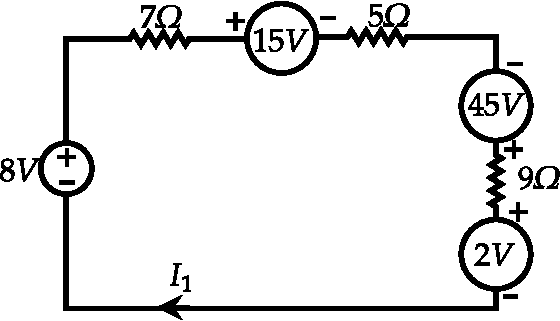
\includegraphics[height=3cm,width=5.3cm]{Ep-5}
		\end{figure}
		\begin{align*}
		\text { Applying KVL }\\
		8-7 I-15-5 I+45-9 I-2 V&=0\\
		53-17-21 \mathrm{I}=0, \quad \mathrm{I}&=\frac{36}{21} \mathrm{I}=1.71
		\end{align*}
	\end{answer}
	\item Calculate the values of $\mathrm{V}_{1}$ and $\mathrm{V}_{2}$ by $\mathrm{KCL}$ :
	\begin{figure}[H]
		\centering
		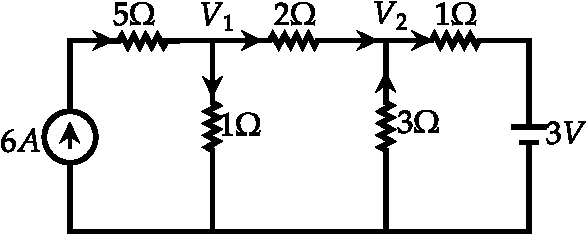
\includegraphics[height=2.5cm,width=6cm]{Ep-6}
	\end{figure}
	\begin{answer}
		\begin{align}
		\text { Applying } \mathrm{KCL} \text { at node } 1: 6&=\frac{V_{1}}{1}+\frac{V_{1}-V_{2}}{2}\label{EP-1}\\
		\mathrm{KCL} \text { at node (2) : } \frac{3-V_{2}}{1}&=\frac{V_{2}}{3}+\frac{V_{2}-V_{1}}{2}\label{EP-2}\\
		\text { By solving equation  }&\text{(\ref{EP-1}) and (\ref{EP-2});}\notag\\
		\text { We get } V_{1}&=5 \mathrm{~V} \text { and } \mathrm{V}_{2}=3 \mathrm{~V}\notag
		\end{align}
	\end{answer}
	\item Obtain single current source for network shown
	\begin{figure}[H]
		\centering
		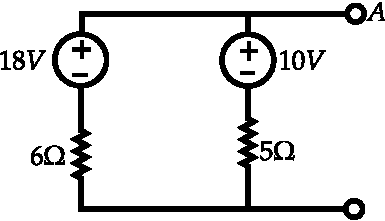
\includegraphics[height=2.5cm,width=4.4cm]{Ep-7}
	\end{figure}
	\begin{answer}
	\begin{figure}[H]
		\centering
		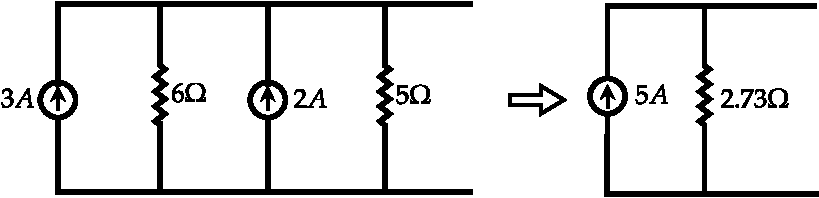
\includegraphics[height=2.5cm,width=9cm]{Ep-8}
	\end{figure}
	\end{answer}
	\item Convert given circuit into a single voltage source
	\begin{figure}[H]
		\centering
		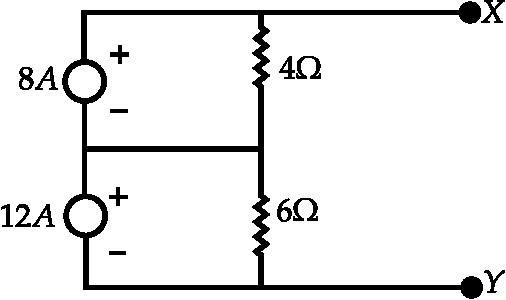
\includegraphics[height=3cm,width=5cm]{Ep-9}
	\end{figure}
	\begin{answer}$\left. \right. $\\
		\begin{figure}[H]
			\centering
			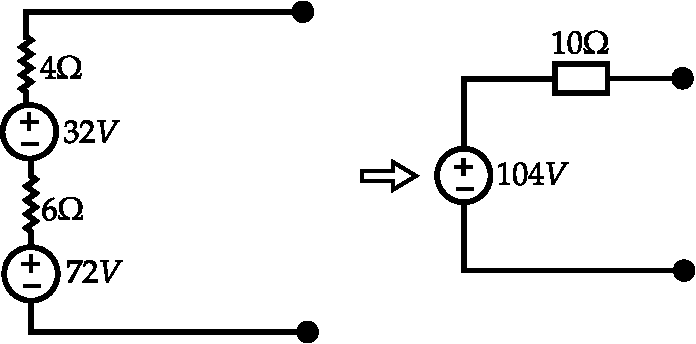
\includegraphics[height=3cm,width=6cm]{Ep-10}
		\end{figure}
	\end{answer}
	\item Calculate value of $V$ for the given circuit by using superposition theorem.\\
	$\mathrm{I}_{\mathrm{eq}}=\mathrm{I}_{1} \pm \mathrm{I}_{2} \pm \mathrm{I}_{3} \ldots \ldots \ldots \pm \pm \mathrm{I}_{\mathrm{n}}$
	\begin{figure}[H]
		\centering
		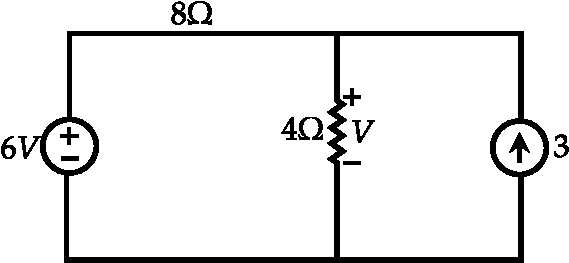
\includegraphics[height=2.5cm,width=5.5cm]{Ep-33}
	\end{figure}
	\begin{answer}
		At one time only effect of one source is considered. Voltage source is short circuited and current source is open circuited.\\
		Since there are two sources, So, $V=V_{1}+V_{2}$\\
		Let $\mathrm{V}_{1}$ is the voltage across 4 ohm due to $6 \mathrm{~V}$ voltage source alone (in this case current source is oper circuited).
		\begin{figure}[H]
			\centering
			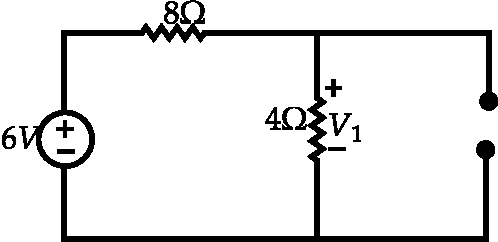
\includegraphics[height=2.7cm,width=5.5cm]{Ep-15}
		\end{figure}
		\begin{align*}
		V_{1}&=\frac{6}{8+4} \times 4, \quad V_{1}=\frac{6}{12} \times 4=2 \mathrm{~V}
		\intertext{Let $\mathrm{V}_{2}$ is the voltage due to $3 \mathrm{~A}$ current source alone (in this case voltage source is short circuited).}
		3&=\frac{V_{2}}{4}+\frac{V_{2}}{8}, \quad 3=\frac{V_{2}}{8}\{2+1\} \quad V_{2}=8 \text { volts }\\
		\text { So total voltage } &\mathrm{V} \text { is } \mathrm{V}=\mathrm{V}_{1}+\mathrm{V}_{2}=2+8=10 \text { volt }
		\end{align*}
		\begin{figure}[H]
			\centering
			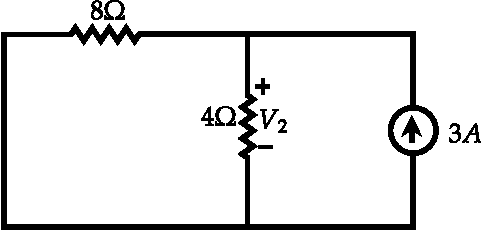
\includegraphics[height=2.7cm,width=5.5cm]{Ep-16}
		\end{figure}
	\end{answer}
	\item Calculate the value of $\mathrm{V}_{0}$ ?
	\begin{figure}[H]
		\centering
		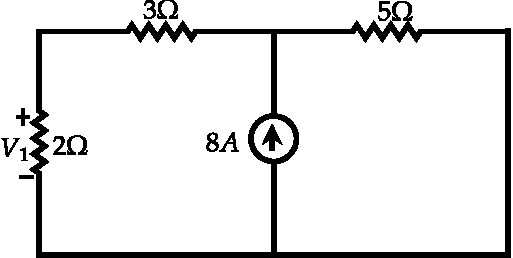
\includegraphics[height=2.5cm,width=5cm]{Ep-17}
	\end{figure}
	\begin{answer}
		Since there are two sources so total voltage due to both sources will be $V_{0}=V_{1}+V_{2}$\\
		Let $\mathrm{V}_{1}$ is the voltage only due to $8 \mathrm{~A}$ current source, (In this case $20 \mathrm{~V}$ source is short circuited)
		\begin{figure}[H]
			\centering
			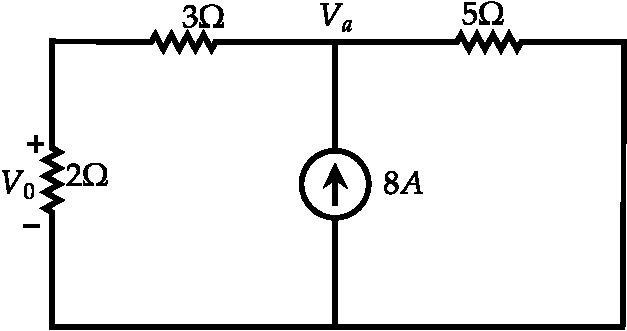
\includegraphics[height=2.7cm,width=5cm]{Ep-18}
		\end{figure}
		\begin{align*}
		-8+\frac{V_{a}}{5}+\frac{V_{a}}{5} &=0 \\
		\frac{2 V_{a}}{5} &=8 \\
		V_{a} &=20 \mathrm{~V} \\
		I_{2 \Omega} &=\frac{V_{a}}{5}=4 \mathrm{amp} \\
		V_{1} &=4 \times 2=8 \text { volt }
		\end{align*}
	\end{answer}
	\item For the given circuit calculate the power loss in the 1 ohm resistor by use of thevenin's theorem.
	\begin{figure}[H]
		\centering
		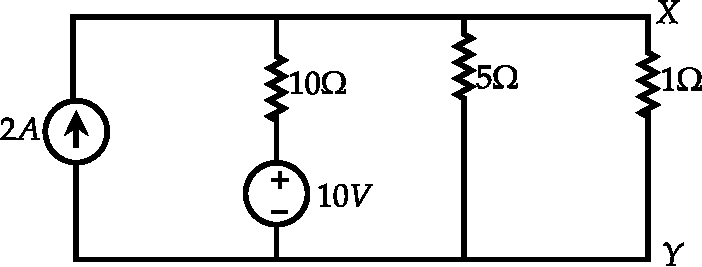
\includegraphics[height=2.3cm,width=6cm]{Ep-19}
	\end{figure}
	\begin{answer}
		For calculation of $\mathrm{V}_{\mathrm{th}}$ branch $\mathrm{X}-\mathrm{Y}$ terminal is assumed as open circuited and let voltage is $\mathrm{V}_{\mathrm{th^-}}$ 
		\begin{figure}[H]
			\centering
			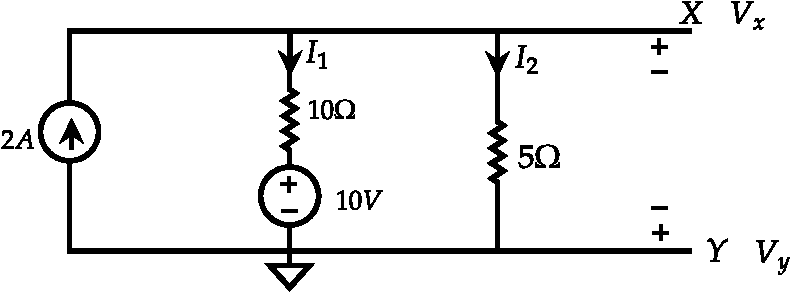
\includegraphics[height=2.7cm,width=6.7cm]{Ep-20}
		\end{figure}
		\begin{align*}
		2&=\mathrm{I}_{1}+\mathrm{I}_{2}, \quad 2=\frac{V_{x}-10}{10}+\frac{V_{x}}{5}, 2=V_{x}\left\{\frac{1}{10}+\frac{1}{5}\right\}-1, V_{x}\left\{\frac{3}{10}\right\}=3 \\
		V_{x}&=10 \text { Volts }, \quad V_{x}-V_{y}=5 \times 2=10 \quad V_{T h}=10 \text { Volt }
		\end{align*}
		\textbf{For Calculation of $\mathbf{R}_{\mathbf{Th}}$ : }(If dependent source is present) $2 \mathrm{~A}$ current source is open circuited and 10 source is short circuited and let resistance is $\mathrm{R}_{\mathrm{Th}}$ :
		\begin{figure}[H]
			\centering
			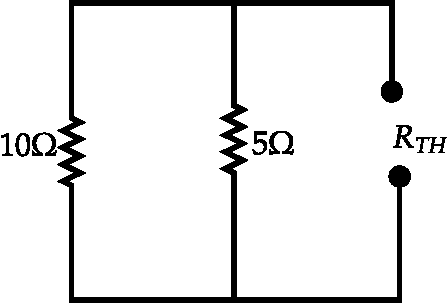
\includegraphics[height=2.5cm,width=3.5cm]{Ep-21}
		\end{figure}
		\begin{align*}
		R_{T h}&=\frac{10 \times 5}{10+5}, \quad R_{m}=\frac{10}{3}=3.3 \Omega\\
		I_{T h}&=\frac{V_{T h}}{R_{T h}+R_{L}}=\frac{10}{3.33+\mathrm{I}}=2.31 \mathrm{~A}
		\end{align*}
	\end{answer}
	\item Find the current through the $5 \Omega$ resistor in the circuit by use of Thevenin's theorem.
	\begin{figure}[H]
		\centering
		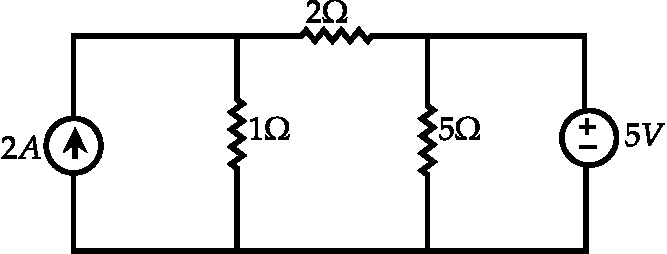
\includegraphics[height=2.7cm,width=6.5cm]{Ep-22}
	\end{figure}
	\begin{answer}
		For calculation of $\mathrm{V}_{\mathrm{Th}}=5 \mathrm{ohm}$ resistor is open circuited and so current in $5 \mathrm{ohm}$ will be zero.
		\begin{align*}
		V_{T h}&=V_{a b}=5 V
		\end{align*}
		\begin{figure}[H]
			\centering
			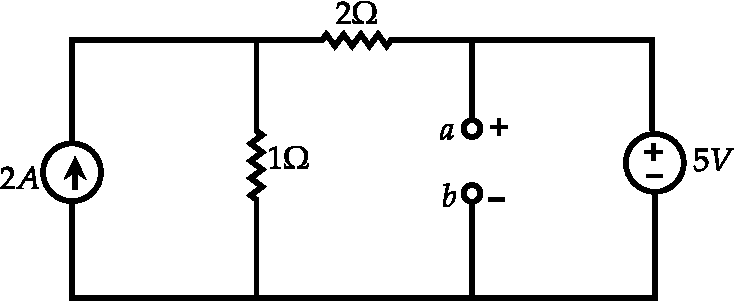
\includegraphics[height=2.7cm,width=6.5cm]{Ep-23}
		\end{figure}
		\textbf{For Calculating $\mathbf{R}_{\mathbf{Th}}$:} $2 \mathrm{~A}$ current source is open circuited and $5 \mathrm{~V}$ source is short circuited.
		\begin{figure}[H]
			\centering
			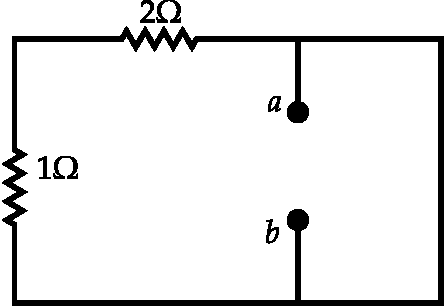
\includegraphics[height=2.7cm,width=3.5cm]{Ep-12}
		\end{figure}
		\begin{align*}
		\mathrm{R}_{\mathrm{Th}}&=\frac{0 \times 3}{3+0}=0, \quad I_{L}=\frac{V_{T h}}{R_{T h}+R_{L}}=\frac{5}{5+10}=1 A
		\end{align*}
	\end{answer}
	\item Find the Norton's equivalent circuit across a-b for the network shown in figure:
	\begin{figure}[H]
		\centering
		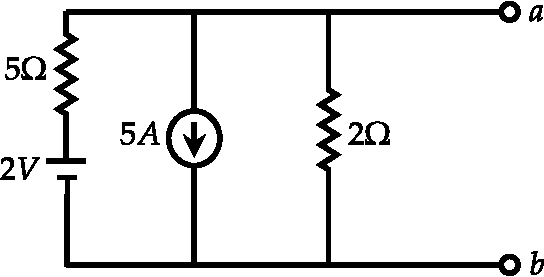
\includegraphics[height=2.7cm,width=5.5cm]{Ep-13}
	\end{figure}
	\begin{answer}$\left. \right. $\\
		\begin{figure}[H]
			\centering
			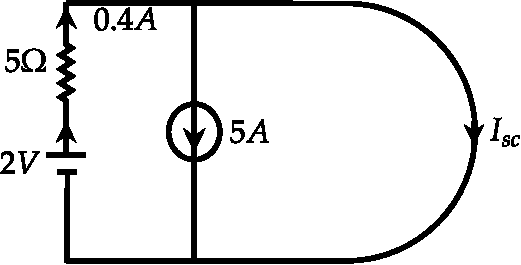
\includegraphics[height=2.7cm,width=5.5cm]{Ep-14}
		\end{figure}
		\begin{align*}
		-2+5\left(5+I_{s c}\right)&=0, I_{s c}=\frac{2}{5}-5=0.4-5 I_{s c}=-4.6 A \\
		R_{T h}&=\frac{2 \times 5}{2+5}=\frac{10}{7} \Omega R_{T h}=1.43
		\end{align*}
	\end{answer}
	\item Find Norton's equivalent to the right of a-b terminal (across $3 \mathrm{~V}$ source)
	\begin{figure}[H]
		\centering
		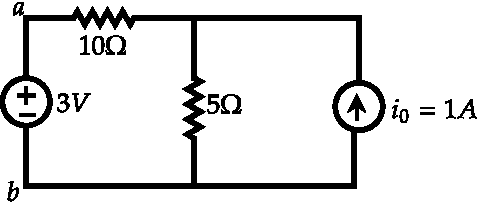
\includegraphics[height=2.5cm,width=5.5cm]{Ep-24}
	\end{figure}
	\begin{answer}
		The equivalent circuit after shorting $a b$ terminal.
		\begin{figure}[H]
			\centering
			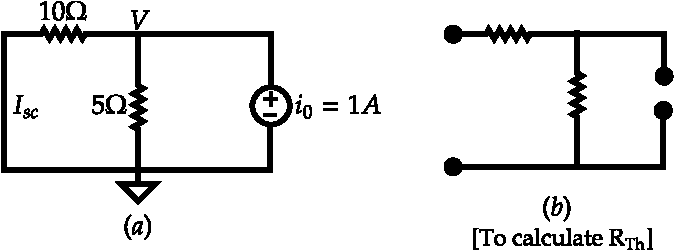
\includegraphics[height=3cm,width=7.5cm]{Ep-25}
		\end{figure}
		\begin{align*}
		\mathrm{i}_{0}&=\mathrm{i}_{1}+\mathrm{I}_{\mathrm{sc}}, \mathrm{I}=\mathrm{i}_{1}+\frac{V}{10} \\
		\mathrm{I}&=\frac{V}{5}+\frac{V}{10}, \mathrm{I}=\frac{3 V}{10}, \mathrm{~V}=\frac{10}{3} \text { and } \mathrm{I}_{\mathrm{sc}}=\frac{1}{3}=0.33 \mathrm{~A} R_{T h}=10+5=15 \Omega
		\end{align*}
	\end{answer}
	\item Calculate value of $R$ in circuit such that maximum power transfer takes place and also calculate amount this power.
	\begin{figure}[H]
		\centering
		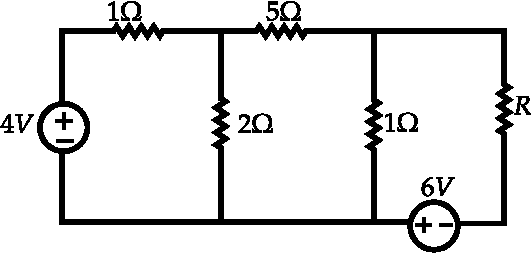
\includegraphics[height=3cm,width=5.7cm]{Ep-26}
	\end{figure}
	\begin{answer}
		\text { Above circuit can be solved by Thevenin's theorem: }
		\begin{figure}[H]
			\centering
			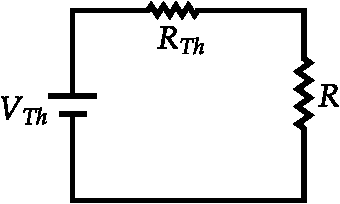
\includegraphics[height=2cm,width=3.2cm]{Ep-27}
		\end{figure}
	To find $R_{Th}$
	\begin{figure}[H]
		\centering
		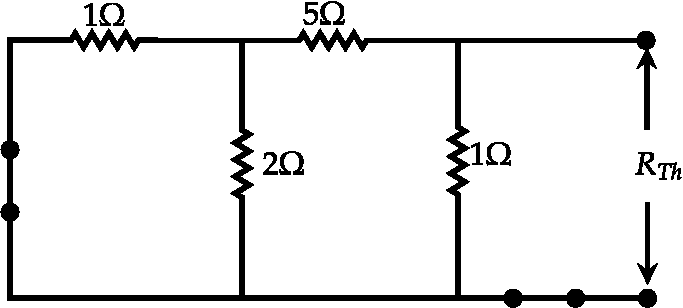
\includegraphics[height=2.8cm,width=5.5cm]{Ep-28}
	\end{figure}
		$R_{T h}=[(2 \| 1)+5] \| 1 \quad R_{T h}=0.85$\\
		To find $V_{T h}$ open load $R$
		\begin{figure}[H]
			\centering
			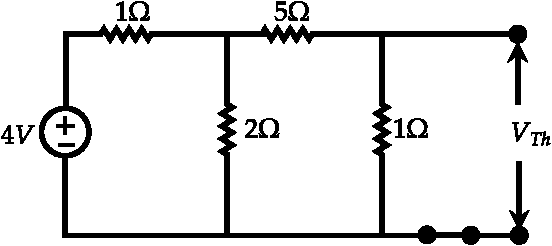
\includegraphics[height=2.8cm,width=5.5cm]{Ep-29}
		\end{figure}
		Maximum Power $=\frac{V_{T h}^{2}}{4 R_{T h}}=\frac{(6.4)^{2}}{4 \times 0.85}=12 \mathrm{~W}$
	\end{answer}
	\item Assuming maximum power transfer from source to load $R$ calculate the value of $R$ and maximum value of power transferred.
	\begin{figure}[H]
		\centering
		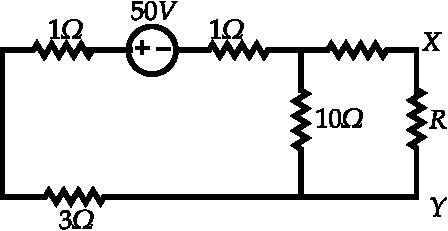
\includegraphics[height=3cm,width=5.5cm]{Ep-30}
	\end{figure}
	\begin{answer}
		\begin{align*}
		\mathrm{V}_{\mathrm{Th}} \text { across } \mathrm{XY}&=-\frac{100}{3} \mathrm{~V}, \mathrm{R}_{\mathrm{Th}} \text { across } \mathrm{XY}=\frac{25}{3} \Omega \\
		\mathrm{P}_{\max }&=\frac{V_{T h}^{2}}{4 R_{T h}}=\frac{(100 / 3)^{2}}{4 \times \frac{25}{3}}=\frac{100}{3} \text { Watt }
		\end{align*}
		\textbf{$\mathbf{R}_{\mathbf{TH}}$ calculation:}
		\begin{figure}[H]
			\centering
			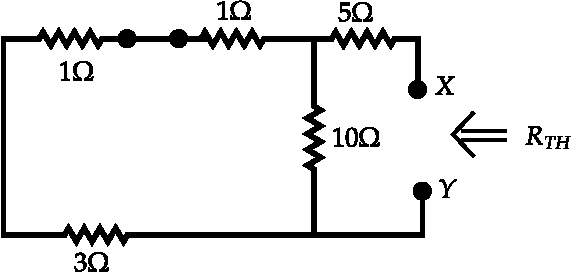
\includegraphics[height=3cm,width=5.8cm]{Ep-31}
		\end{figure}
		\textbf{$\mathbf{V}_{\mathbf{TH}}$ Calculation:}
			\begin{figure}[H]
			\centering
			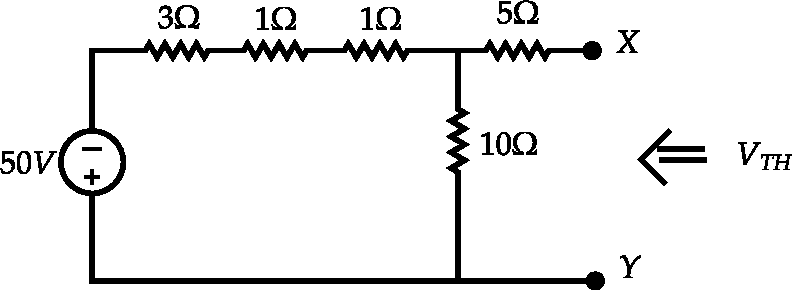
\includegraphics[height=2.8cm,width=6.8cm]{Ep-32}
		\end{figure}
	\end{answer}
\end{enumerate}